% This document is made freely avaiable through the CC0 1.0 Universal license (logo excluded).
% Similar material avaiable at https://github.com/noahhaworth/CAD_Material
% Things to fix:
%		make wording more accurate + spelling check
%		consider adding color
%		increase dimension size fig4
%		ensure all figures are well defined

\documentclass{article}
\usepackage[utf8]{inputenc}
\usepackage[legalpaper, landscape,top=.5in,right=1.5in,left=1.5in,bottom=1.5in]{geometry}
\usepackage{ragged2e}
\usepackage{graphicx}
\usepackage{float}
\usepackage{setspace}
\usepackage[labelfont=bf]{caption}
\usepackage{hyperref}
\usepackage{array}
\usepackage{xcolor}
\hypersetup{colorlinks=true, urlcolor=blue}

\begin{document}
\definecolor{noah}{HTML}{ffffff}
\pagecolor{noah}
\center
\Huge{\textbf{AutoCAD Practice Problems}}\\[3mm] \hrule
\vspace{4mm}
\includegraphics[width=0.15\textwidth]{~/Documents/github/nwh.png}\\[4mm] 
\justify\normalsize
\textbf{Information:} The following problems were originally part of a three hour AutoCAD exam. You are free to do as you please with this document. More material similar to this can be found \href{https://github.com/noahhaworth/CAD_Material}{here}.\\[10mm]
\newpage
\newgeometry{top=.5in,right=1.5in,left=1.5in,bottom=1.5in}

%problem 1
\textbf{P1}
\begin{figure}[H]
  \centering
  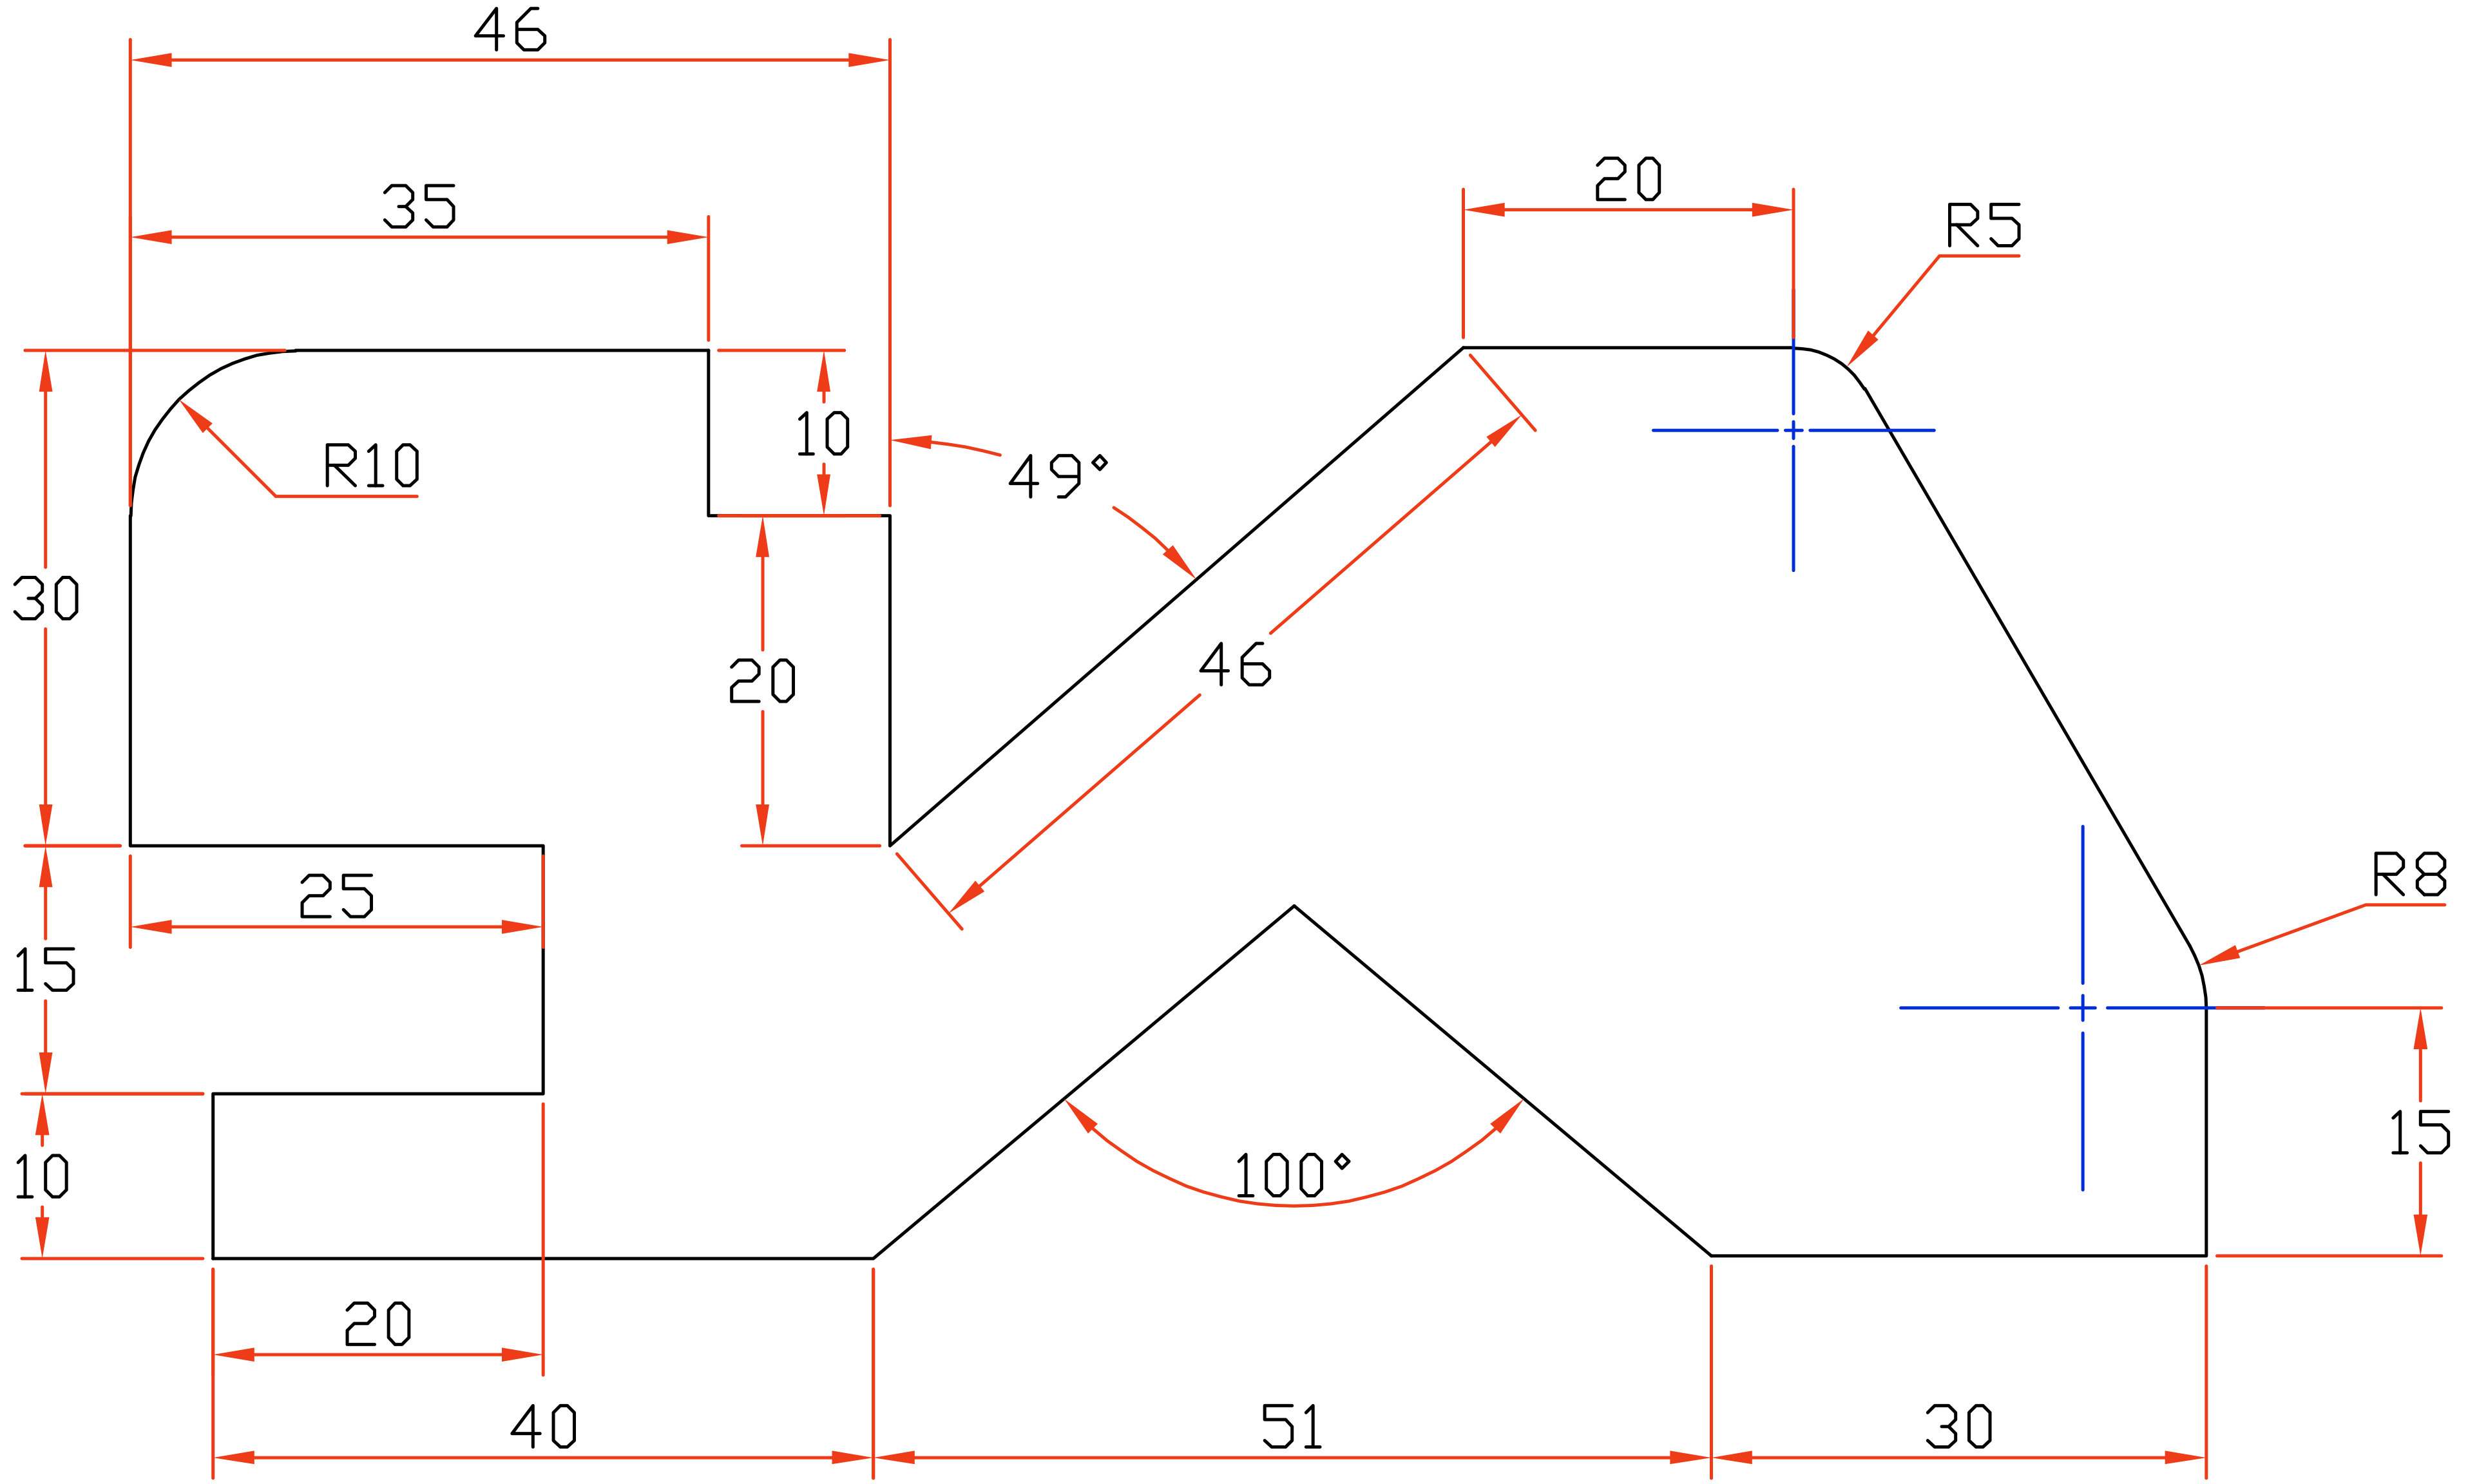
\includegraphics[width=.84\linewidth]{images/1.png}  
  \caption{Sketch 1}
  \label{fig:1}
\end{figure}
\noindent Please create the sketch seen in \textit{Figure 1} in AutoCAD with clear dimensioning. Include the centerlines and centermarks seen in a ``centerline" layer.

%problem 2
\textbf{P2}
\begin{figure}[H]
  \centering
  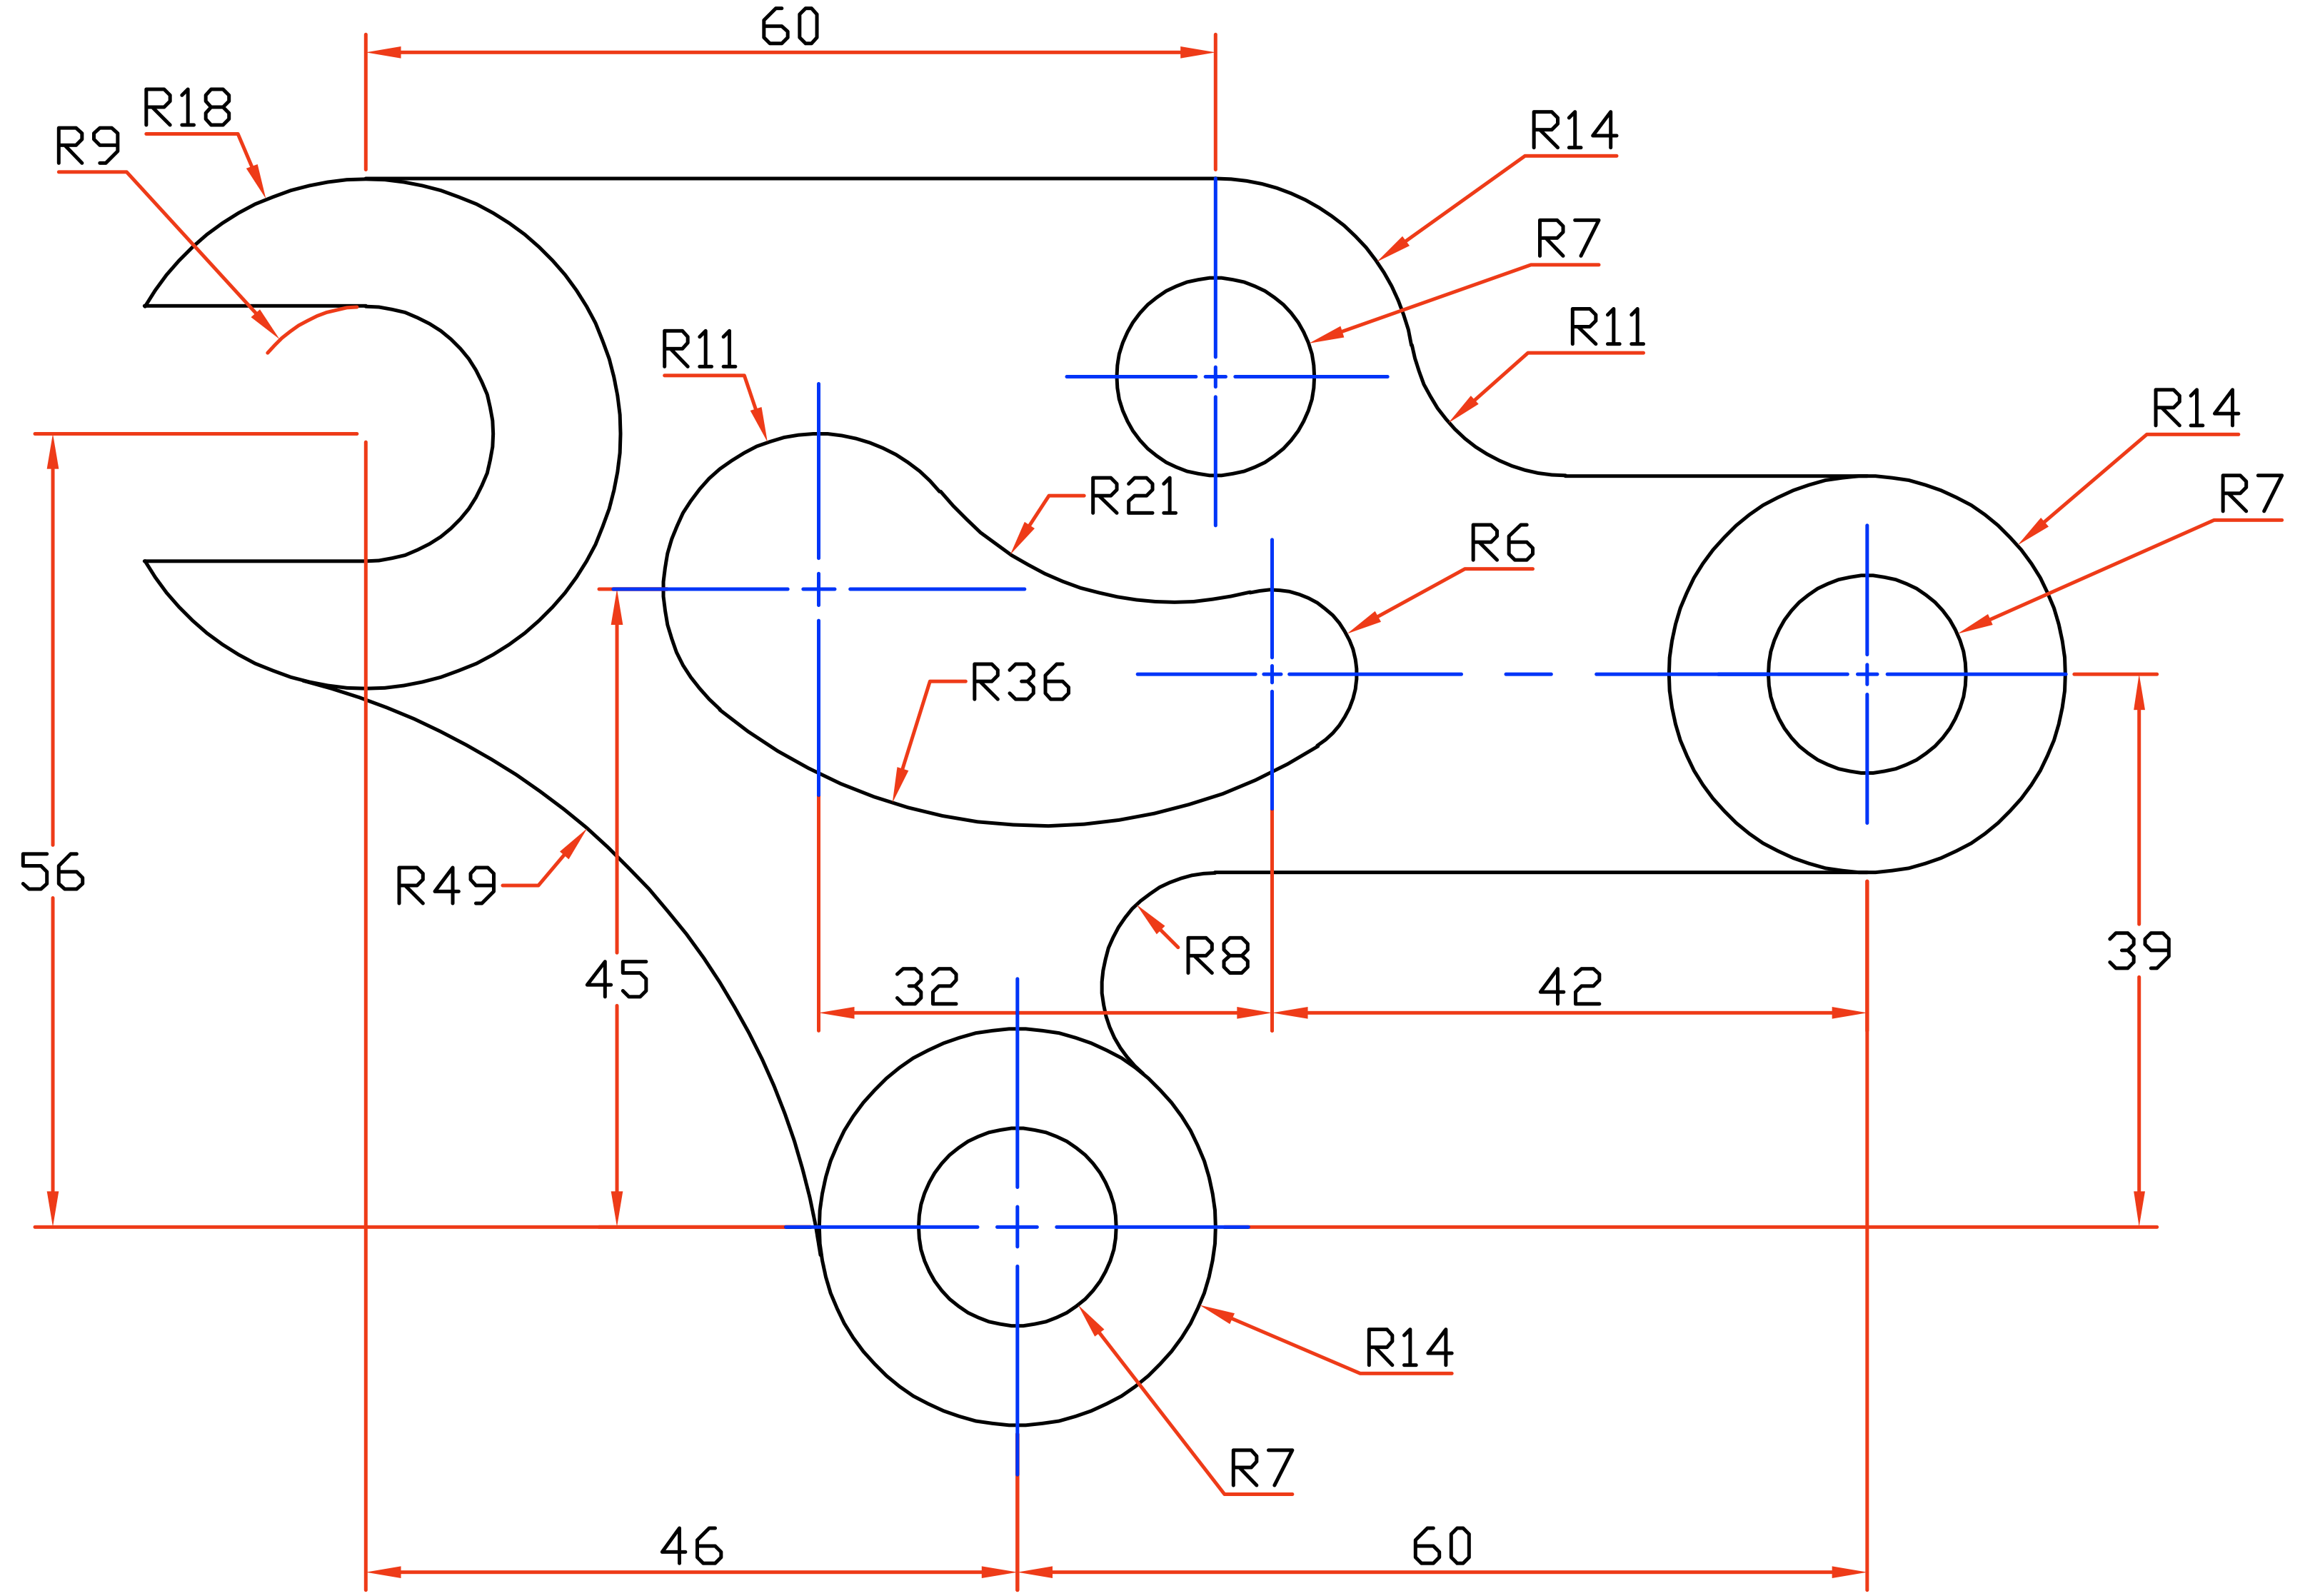
\includegraphics[width=.72\linewidth]{images/2.png}  
  \caption{Sketch 2}
  \label{fig:2}
\end{figure}
\noindent Please create the sketch seen in \textit{Figure 2} in AutoCAD with clear dimensioning. Please include the centermarks seen in a ``centerline" layer.

%problem 3
\textbf{P3}\\
\begin{minipage}[T]{.6\linewidth}
\begin{figure}[H]
  \centering
  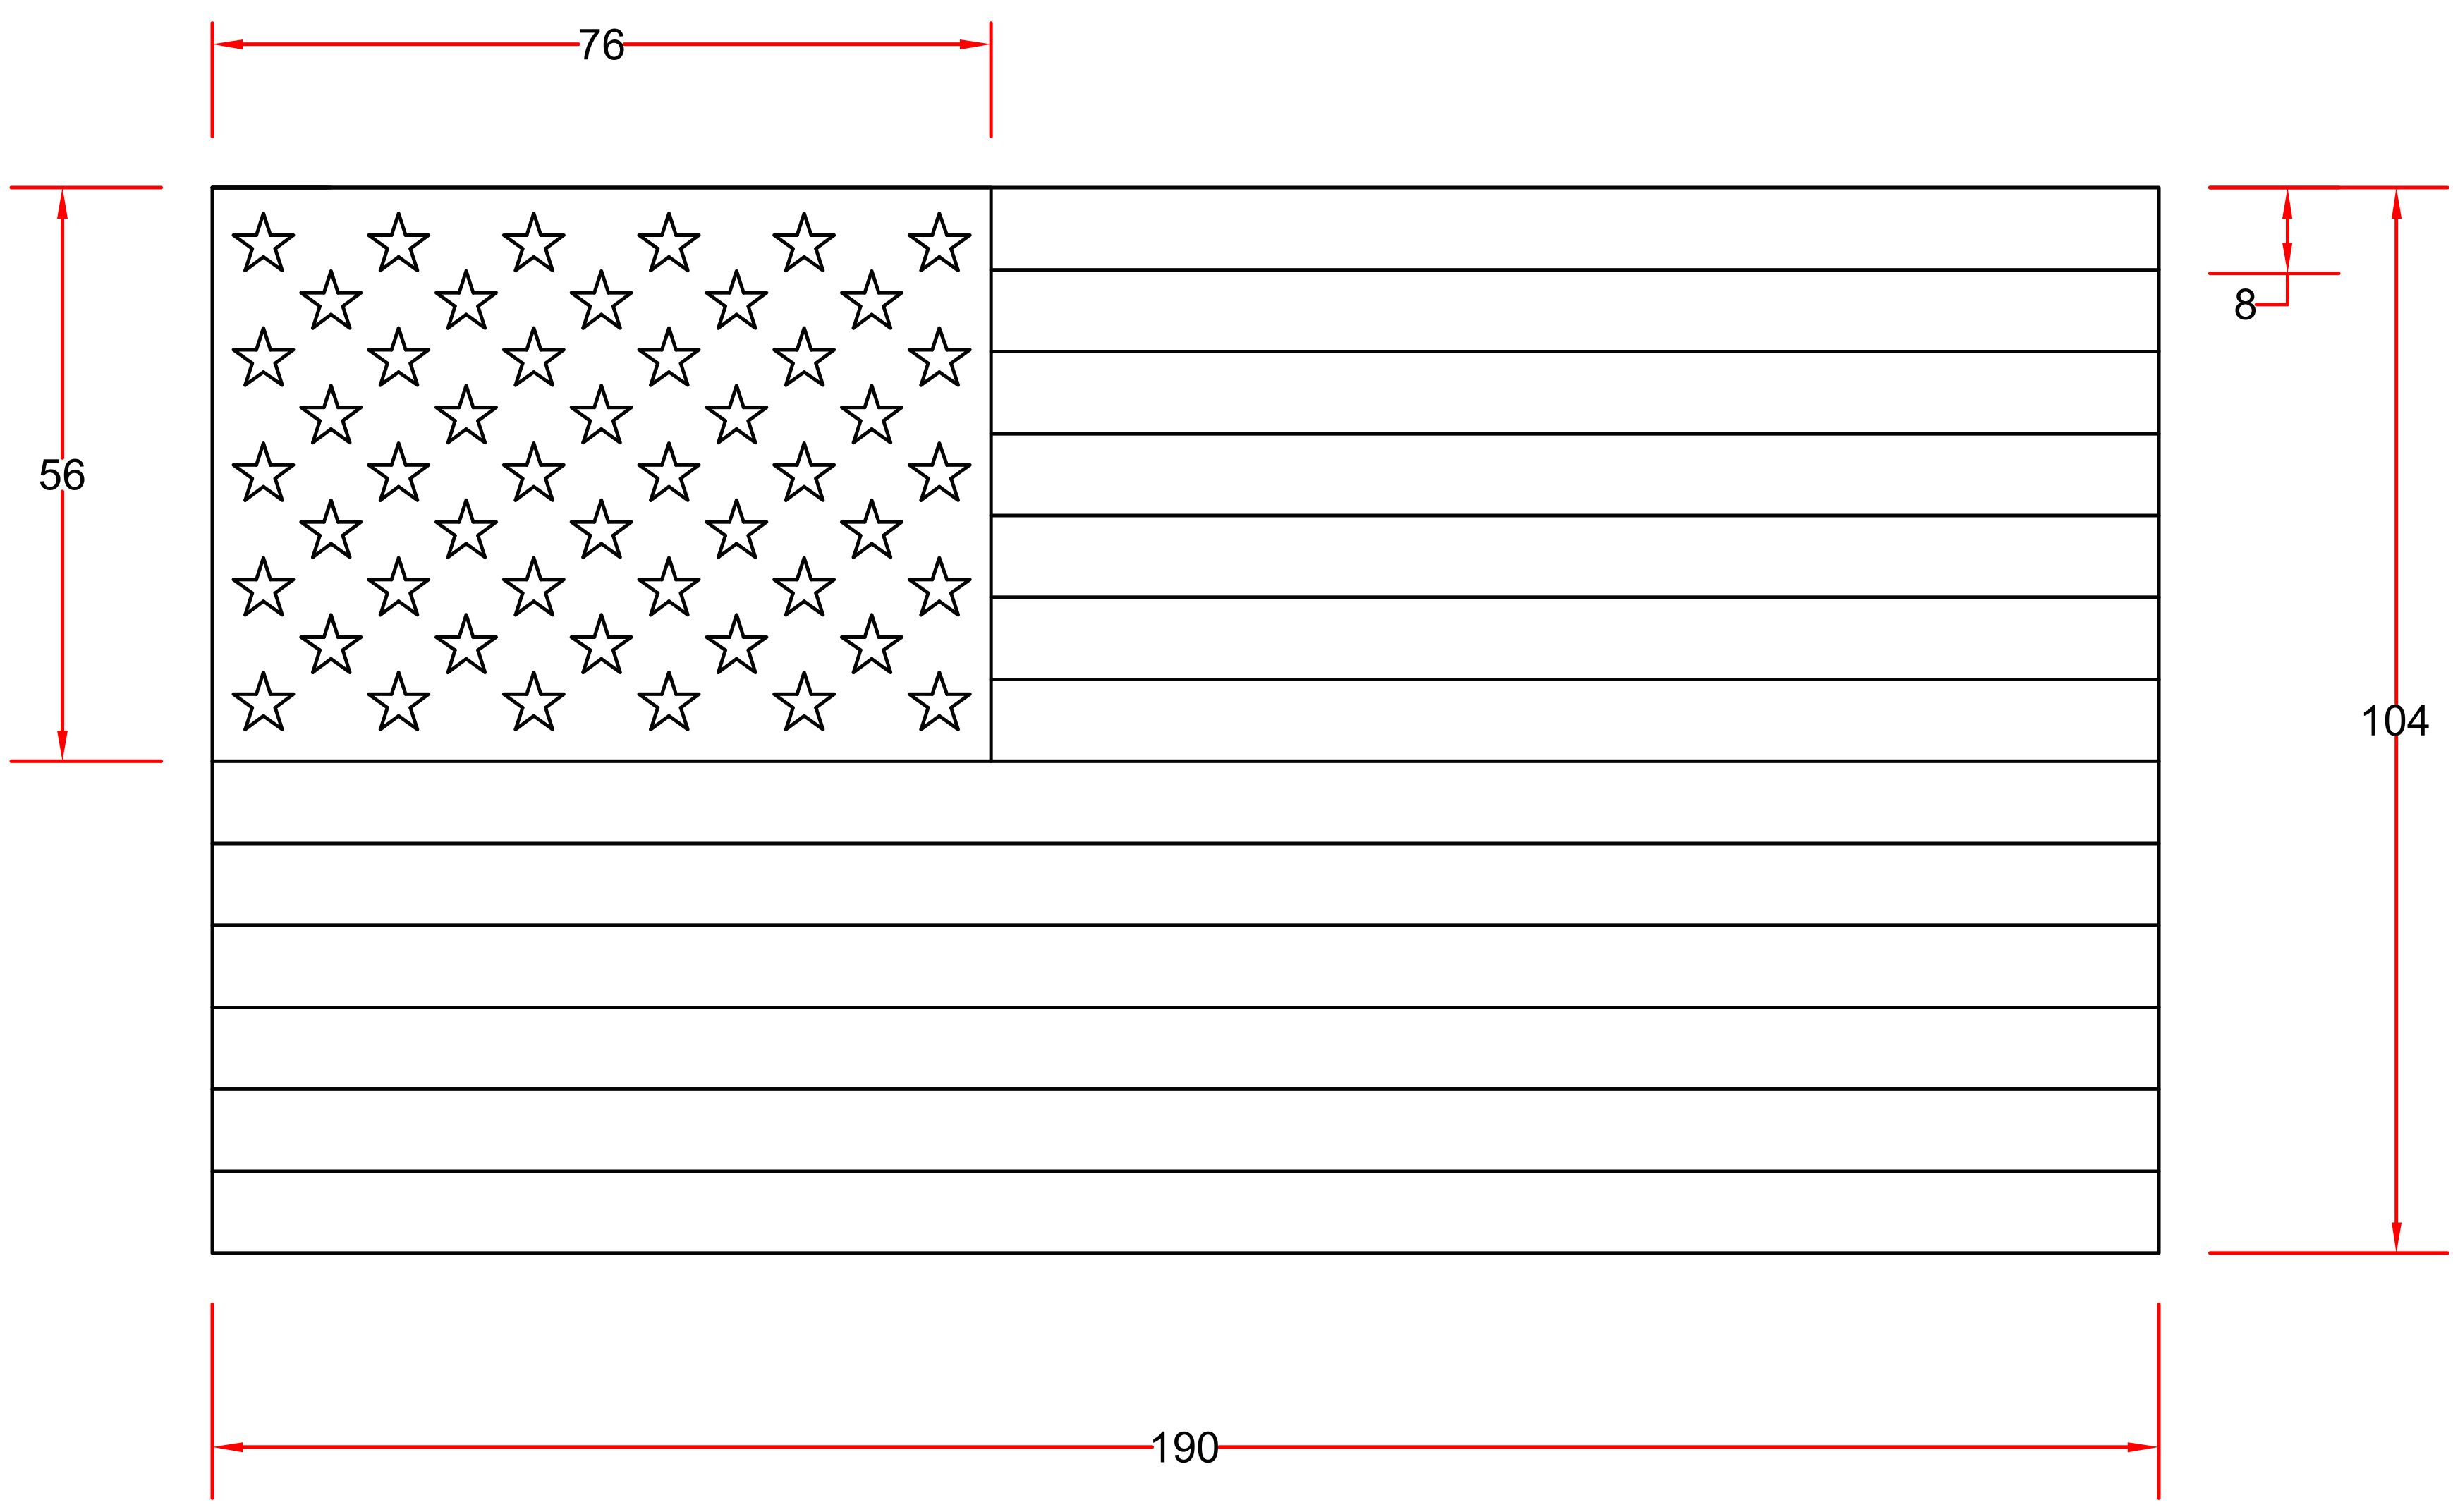
\includegraphics[width=.9\linewidth]{images/3a.png}  
  \caption{Body 1}
  \label{fig:3}
\end{figure}
\end{minipage}
\begin{minipage}[c]{.4\linewidth}
\begin{figure}[H]
  \centering
  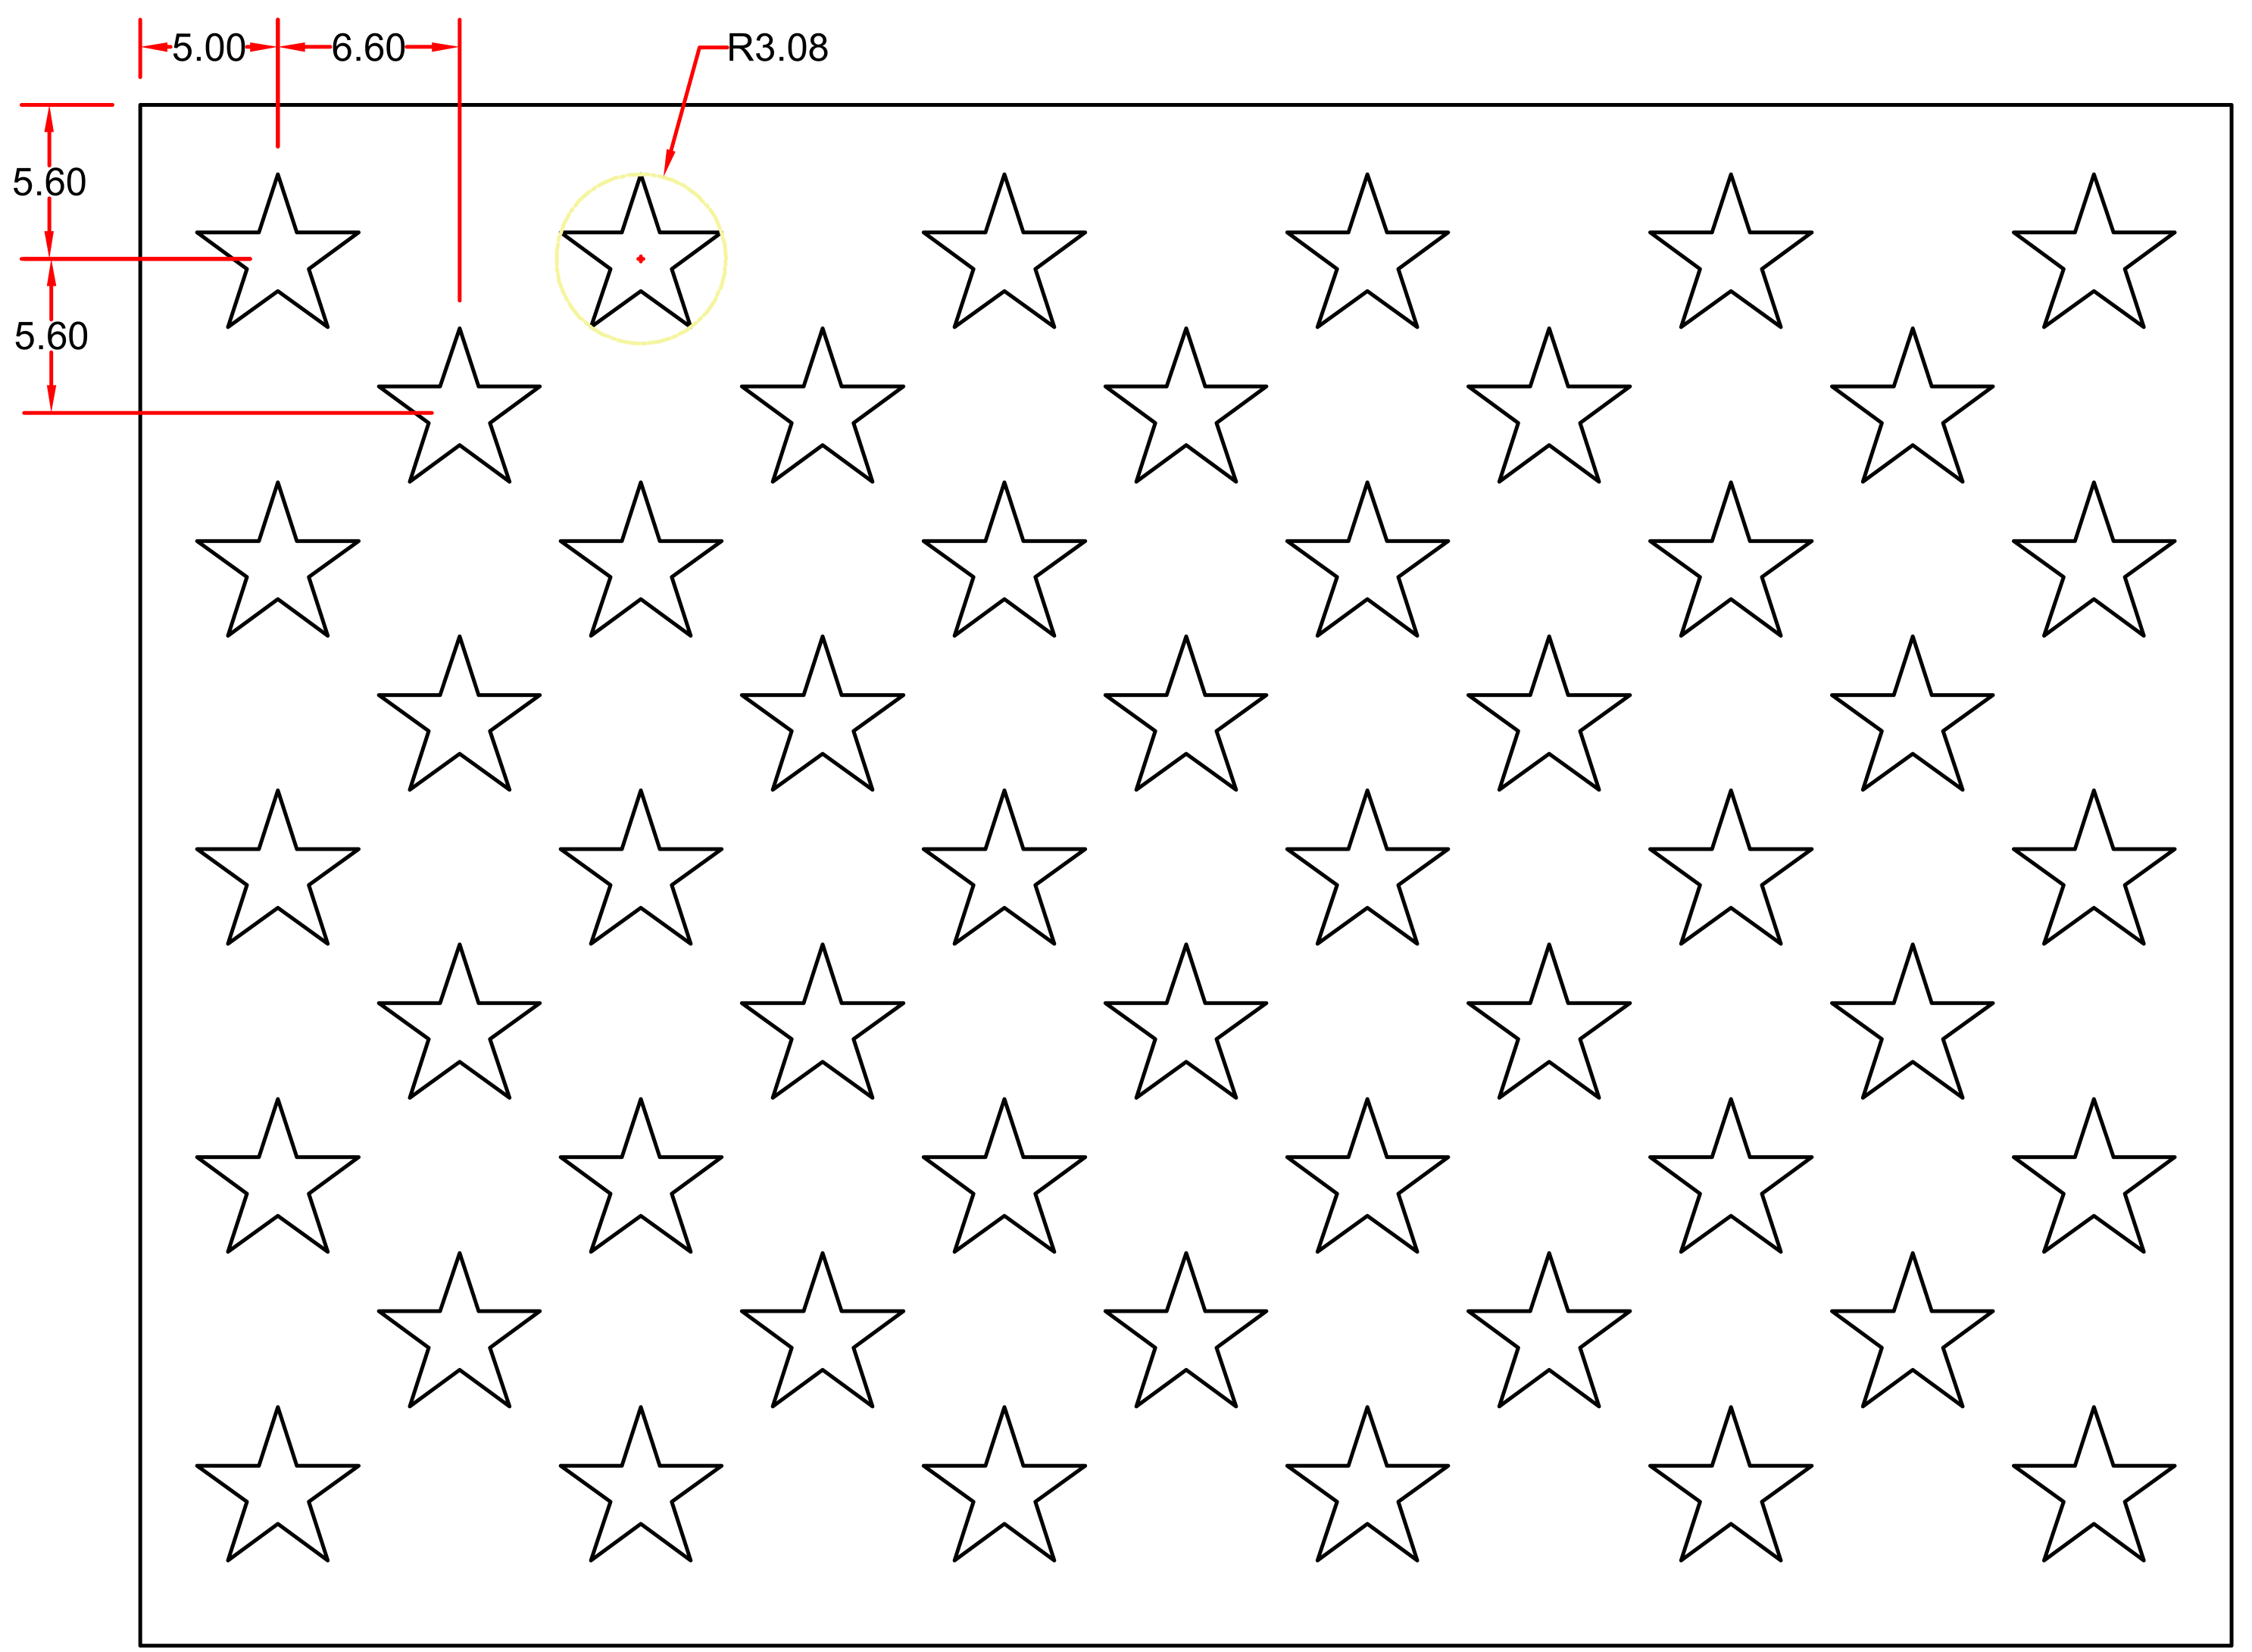
\includegraphics[width=\linewidth]{images/3b.png}  
  \caption{Dimensions}
  \label{fig:4}
\end{figure}
\begin{figure}[H]
  \centering
  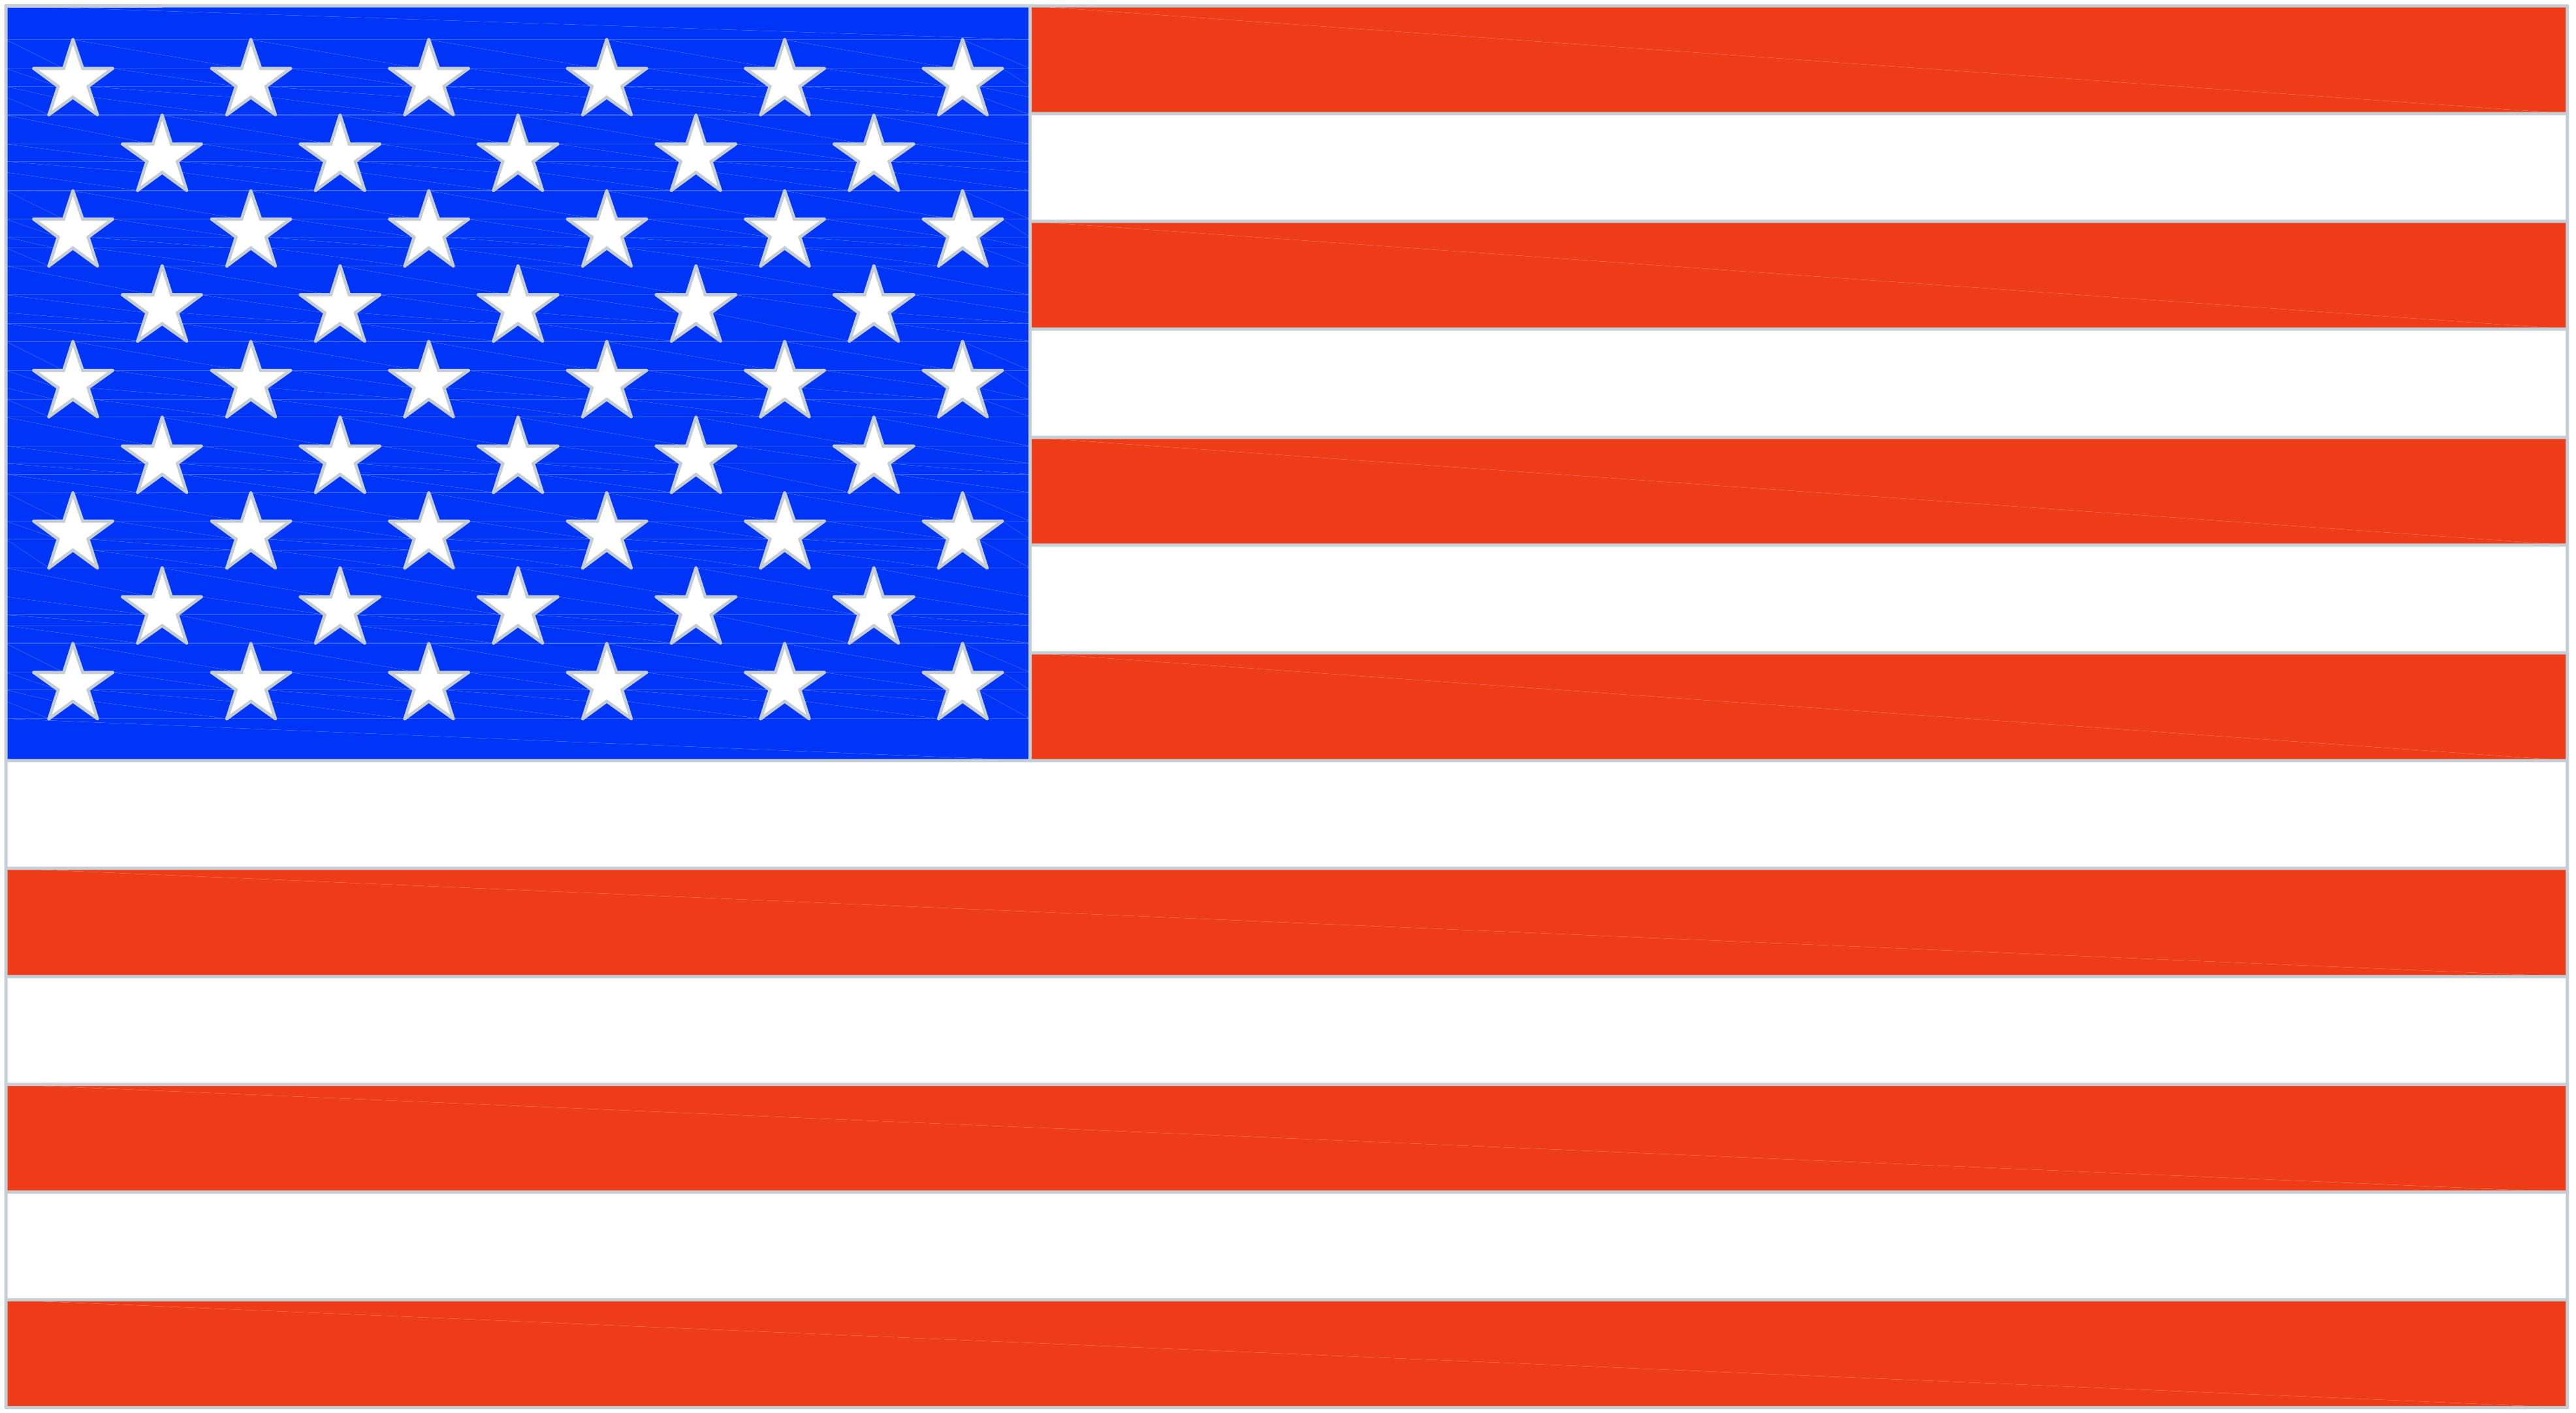
\includegraphics[width=.6\linewidth]{images/3c.png}
  \caption{Colored}
  \label{fig:5}
\end{figure}
\end{minipage}

\vspace{6mm} \noindent Please create a 2D sketch of the flag seen in \textit{Figure 3}. No dimensioning is required. Note that \textit{Figure 4} shows a detailed view of the stars’ repeating pattern. You can use hatching to colorize the flag (as seen in \textit{Figure 5} for extra credit (5 points).

%problem 4
\textbf{P4}
\begin{figure}[H]
  \centering
  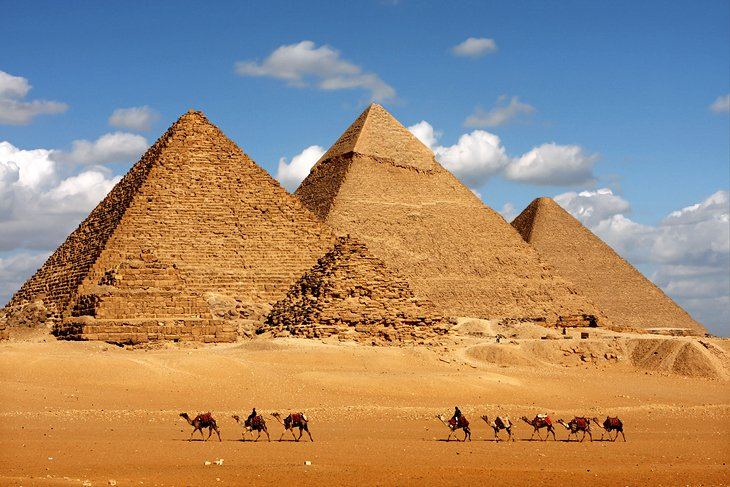
\includegraphics[width=.725\linewidth]{images/4.jpg}  
  \caption{Giza Site}
  \label{fig:6}
\end{figure}
\noindent This problem is optional for extra credit. Please look up the dimensions of the Great Pyramid, the Second Pyramid, and the Third Pyramidand create them in 3D to scale in AutoCAD. No dimensioning is required. Note that the pyramids should be located correctly relative to each other.
\end{document}
